\section*{Side-Chain Entropy in Protein Design}
\label{sec:side_chain_entropy_in_protein_design}
Another approach to the question of side-chain entropy, and one that has only become feasible with recent advances, is to look at its role in the \emph{de novo} design of proteins. The prospect of explicitly calculating all of the thermodynamic parameters involved in folding a protein is already a daunting challenge. Performing these calculations while iterating through all of sequence space to find a specific protein fold is flat out impossible. For that reason, \emph{de novo} design algorithms make simplifying assumptions about what sorts of thermodynamic parameters are important in determining a protein's shape. Most of these algorithms will randomly iterate through sequence space, stopping at regular intervals to minimize the protein structure (for example, by simulated annealing) followed by calculation of scoring function which will determine if the structure should be kept or rejected.

RosettaDesign is just such an algorithm, and Hu and Kuhlman have used it to investigate the role of side-chain entropy in the \emph{de novo} design process\cite{Hu:2006p68}.

\begin{figure}[h]
	\center
	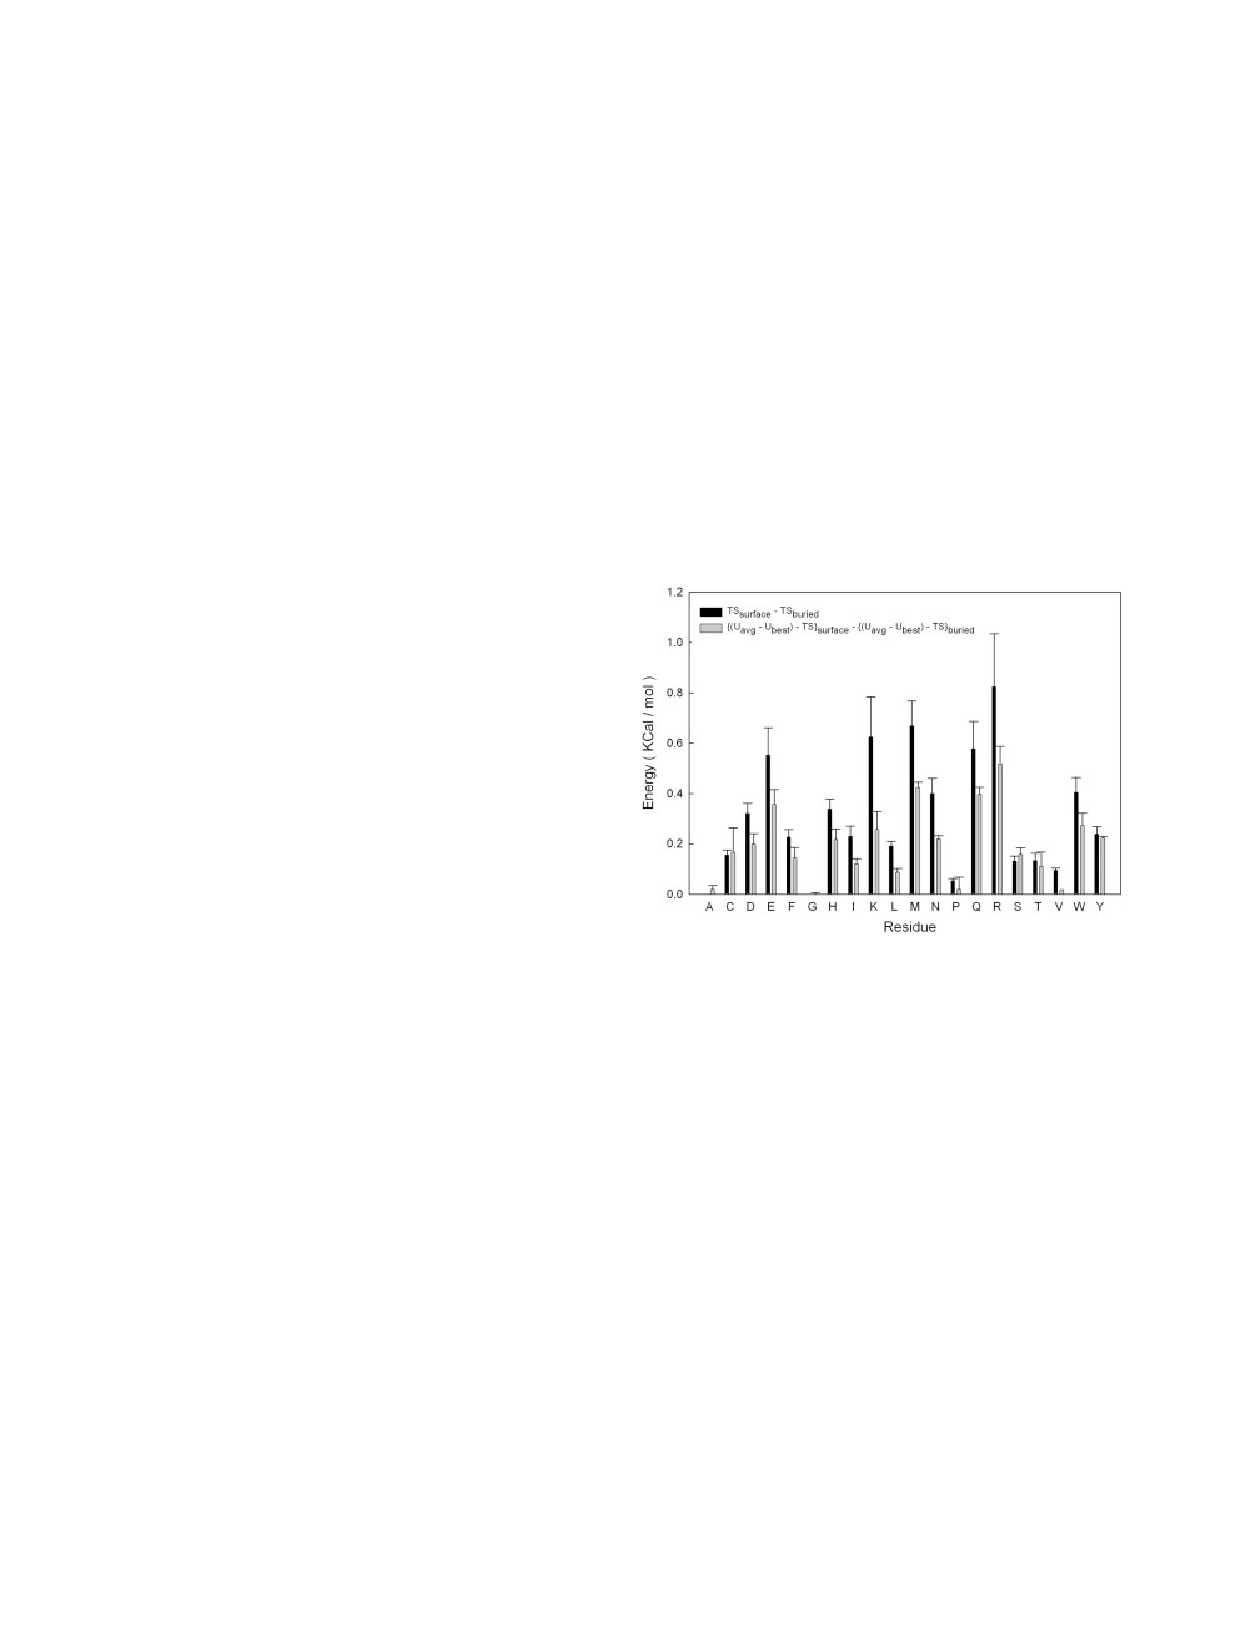
\includegraphics{surface_vs_buried}
	\caption{(Borrowed from \cite{Hu:2006p68}) Changes in side-chain conformational entropy and free energy between surface and buried positions. The black bars show the change in entropy (TS) when a residue is buried whereas the gray bars compare average free energies ($\mathrm{U_{avg}}$ - TS) obtained with the explicit side-chain entropy model to the energies that are calculated with the standard RosettaDesign model ($\mathrm{U_{best}}$). The gray bars indicate the net effect that the explicit side-chain entropy model has on the environmental preferences of the amino acids.}
	\label{fig:surface_vs_buried}
\end{figure}

\begin{itemize}
	\item Review logic
	\item Background on method
	\item Summarize conclusions
	\item Compare to new paper with contradictory results
\end{itemize}
